\chapter{Studies with the Soft Muon Tagger}
Analyses that involve final states with $b$-quarks heavily rely on the accurate identification of these quarks. Ongoing efforts are dedicated to refine this identification process. This chapter presents a study on how muons can contribute to the identification of $b$-quarks in current $b$-tagging algorithms applied to small-$R$ jets. 


\section{Soft Muon tagging}
\label{sec:SoftMuonTagging}
Algorithms currently in use for $b$-tagging described in section \ref{sec:b_tagging}, primarily exploit the displaced secondary vertex that is characteristic of the long lifetime of $b$-quarks. Besides vertex finding algorithms muons can be used as indication for the presence of a $b$-hadron.This is because approximately \qty{20}{\percent} of the $b$-jets undergo semi-leptonic decays that involve a muon as exemplified in figure \ref{fig:semileptonicDecay}. The branching fractions for these decays are roughly \qty{11}{\percent} for direct $b$ to muon decays $BR( b \rightarrow \mu \nu X )$ and about \qty{10}{\percent} for cascade decays $BR( b \rightarrow c \rightarrow \mu \nu X )$ \citep{expectedPerformanceAtlas}.
\begin{figure}[htbp]
  \centering
  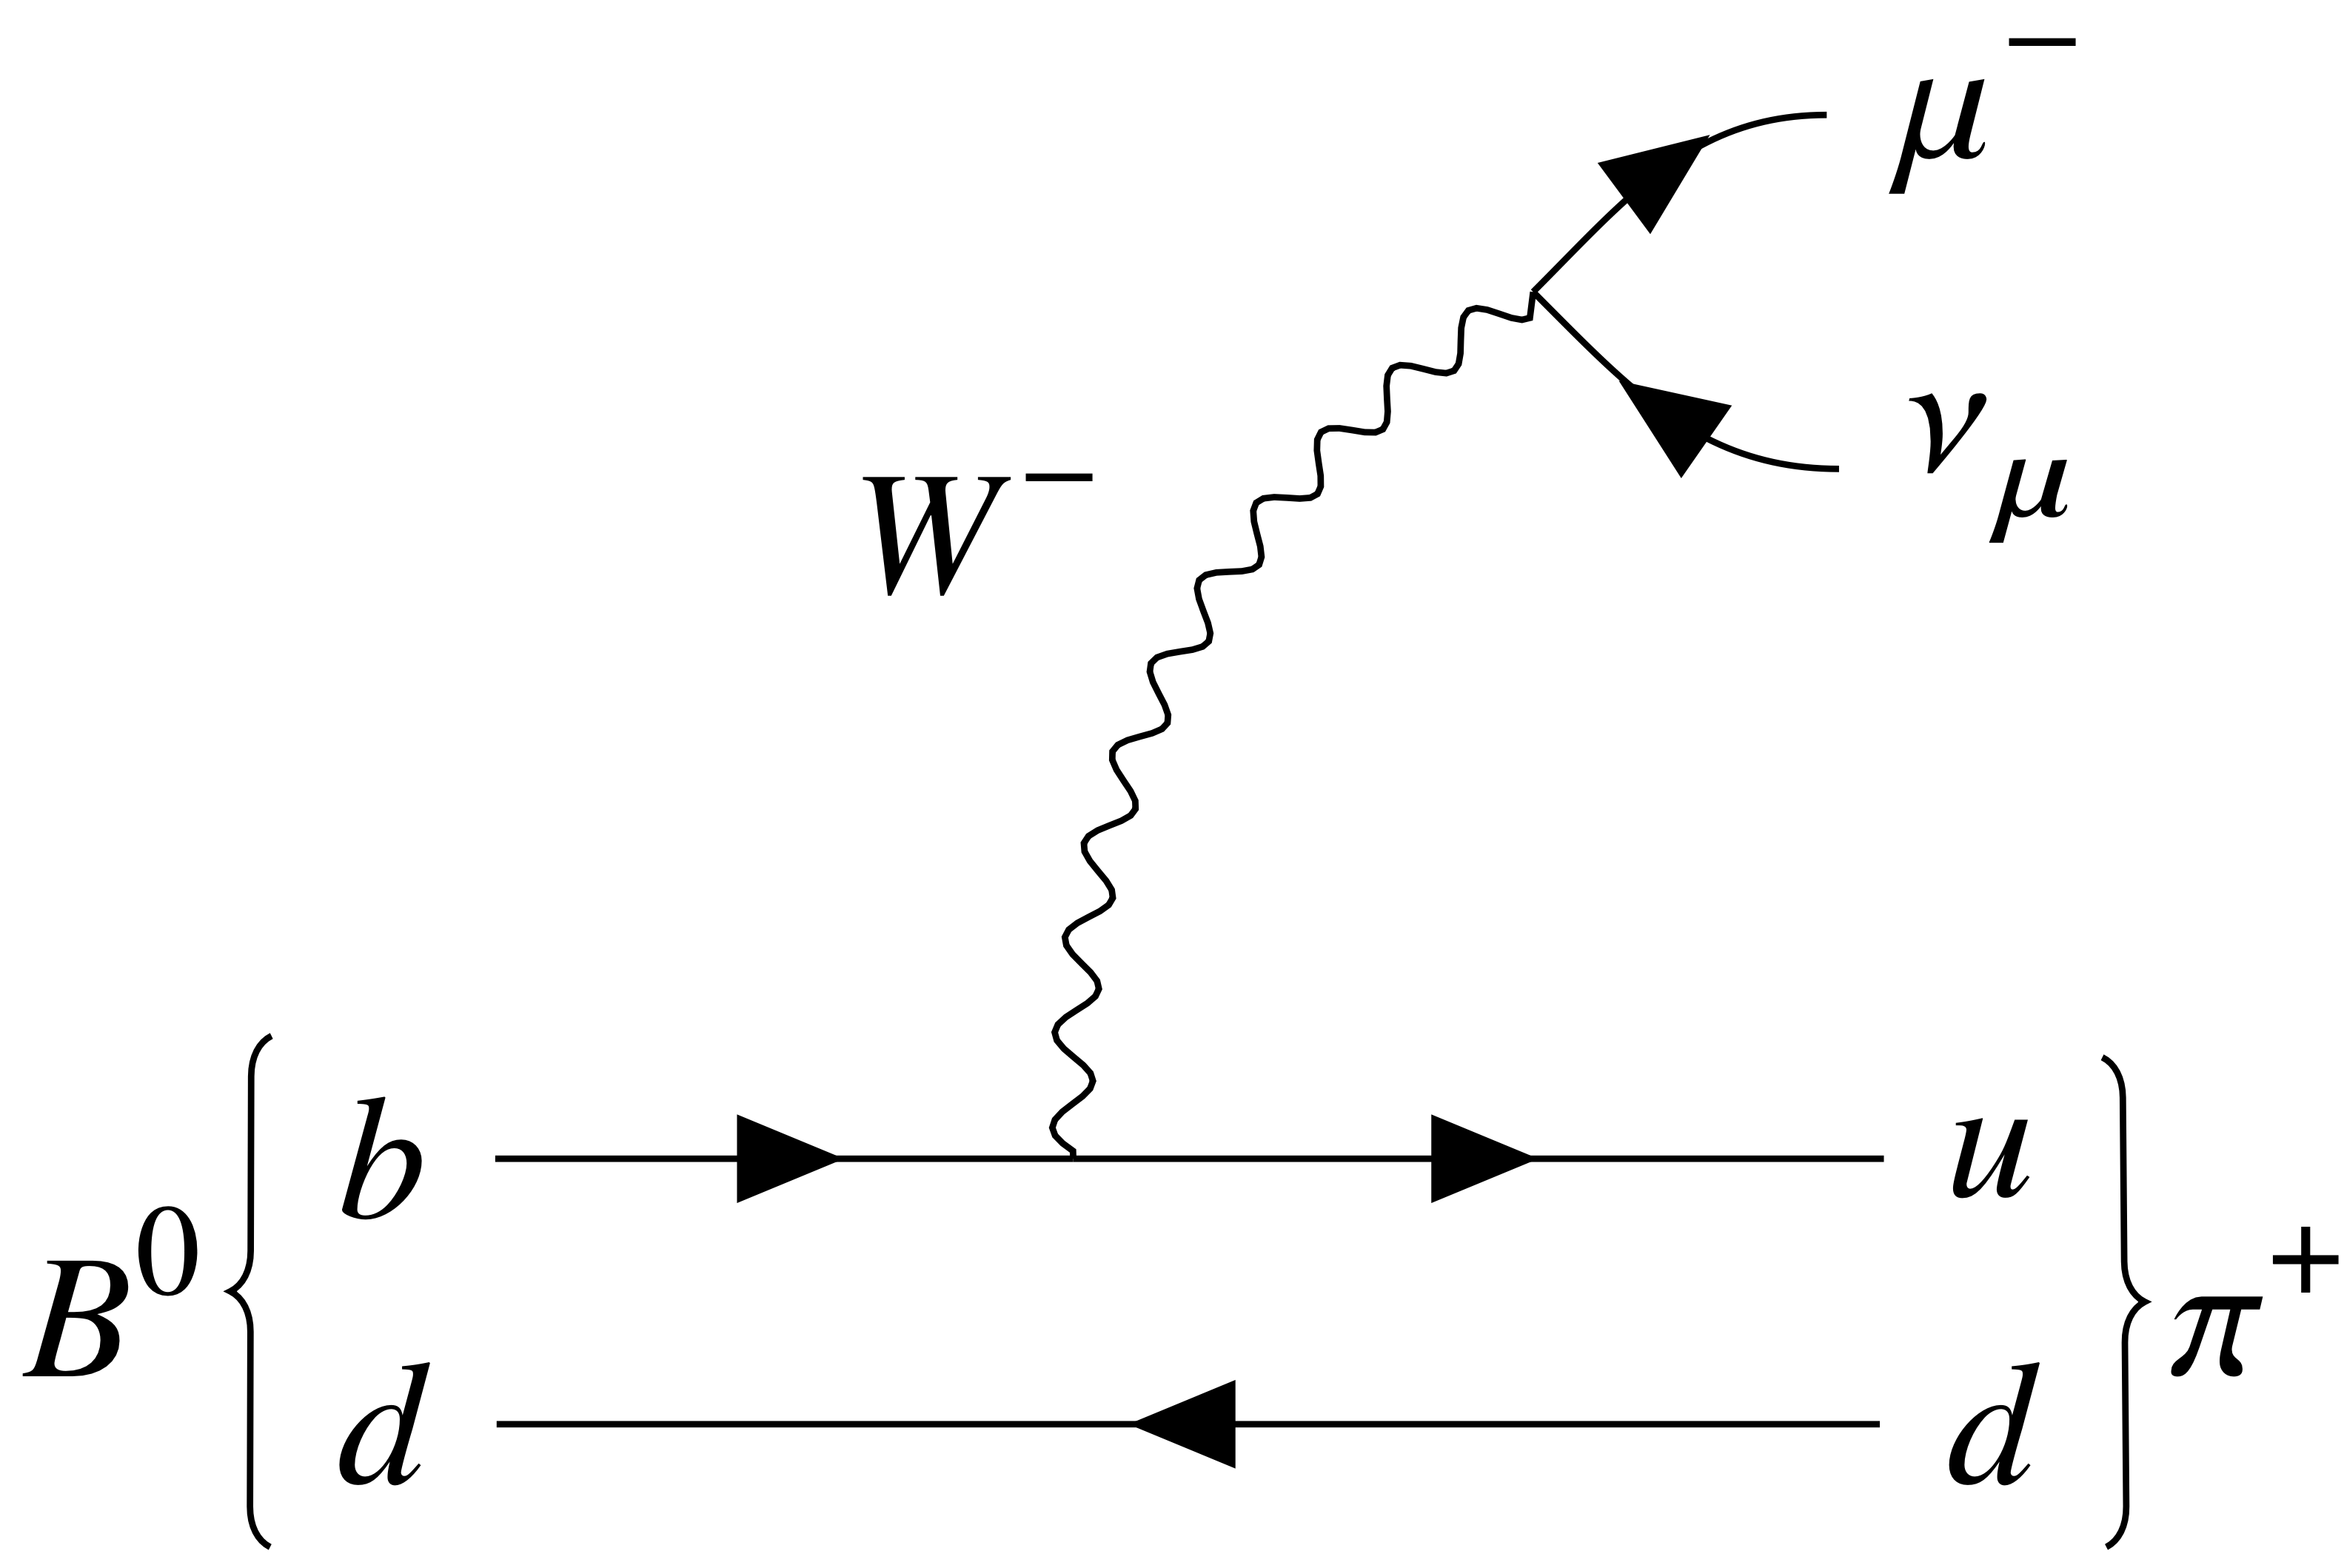
\includegraphics[width=0.4\textwidth]{semileptonic_b_decay}
  \caption{Feynman Diagram depicting a typical semi-leptonic decay of an Anti-$B^0$-meson containing a muon in the final state.}
  \label{fig:semileptonicDecay}
\end{figure}

Despite their limited branching ratio, muons from semi-leptonic heavy-flavor decays are valuable in complementing impact parameter- and vertex-based $b$-tagging methods. These muons typically exhibit higher transverse momentum compared to those from lighter hadron decays, as shown in figure \ref{fig:softMuon_pt}. This relates also to the fact that muons from $b$-decays tend to be more boosted transverse to the jet axis and therefore have a larger orthogonal projection $p_\text{T}^\text{rel}$ of the muon-\pt onto the jet axis. This is calculated by taking the perpendicular part of the three vector muon-momentum to the three-vector jet momentum. The term ``soft'' is derived from the fact that their \pt is smaller than that typically possessed by muons from electroweak boson decays, since they originate from a secondary process \citep{ATL-PHYS-PUB-2017-013}.
\begin{figure}[htbp]
  \centering
  \subfigure[]{
    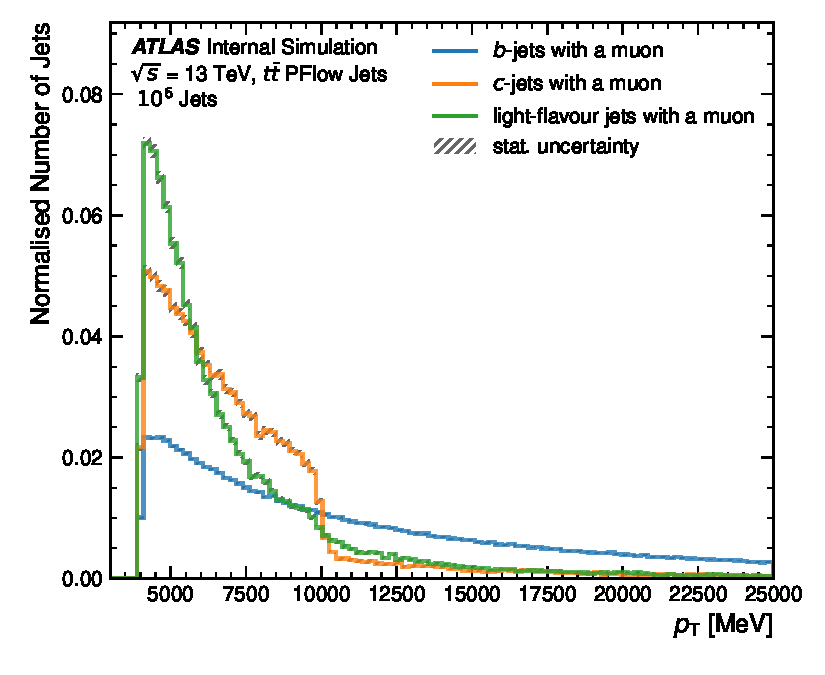
\includegraphics[width=0.45\textwidth]{softMuon_pt}
    \label{fig:softMuon_pt}
  }\hspace*{0.5cm}
  \subfigure[]{
    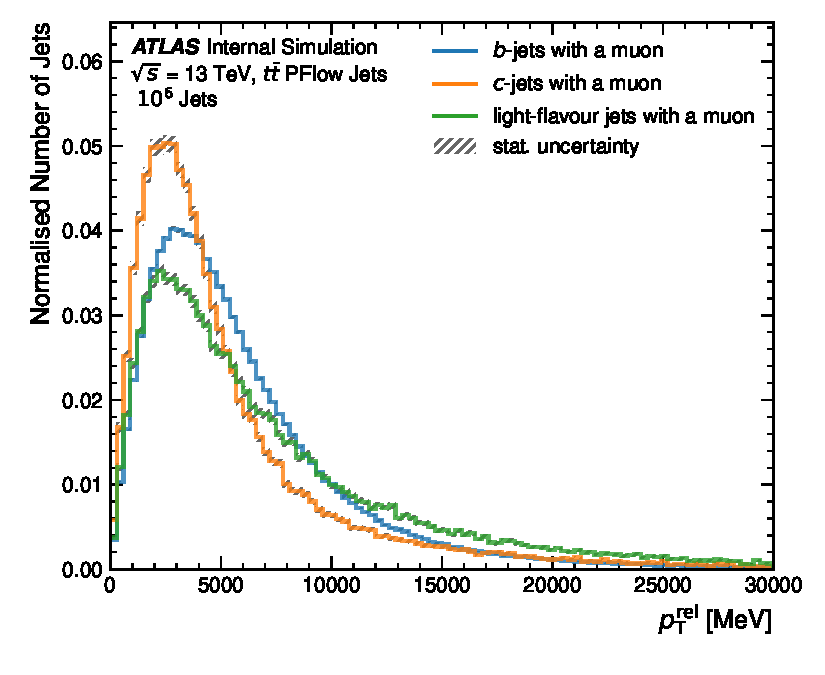
\includegraphics[width=0.45\textwidth]{softMuon_pTrel}
    \label{fig:softMuon_pTrel_sketch}
  }\\
  \subfigure[]{
    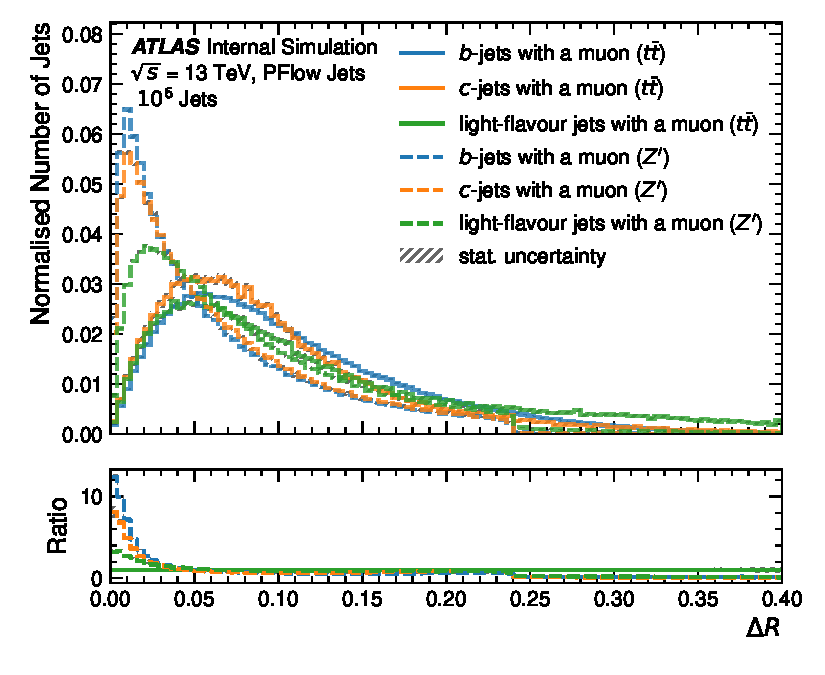
\includegraphics[width=0.49\textwidth]{softMuon_dR}
    \label{fig:softMuon_dR}
  }
  \caption{Kinematics of soft muons: \textbf{(a)} transverse momentum distribution, \textbf{(b)} relative transverse momentum ($p_\text{T}^\text{rel}$) indicative of muons from direct $b$-jet decays being more boosted transversely to the jet axis, and \textbf{(c)} $\Delta R$ distribution between soft muons and jets, normalized per flavor.}
  \label{fig:muonsForSMT}
\end{figure}



% ---------------------------
\section{Muon Selection}
\label{sec:MuonSelection}
%-------------------------------------------------------------------------------
The particle flow algorithm used to reconstruct small-$R$ jets described in section \ref{sec:particle_flow} does not include muons. To address this muons are associated to jets using the shrinking association \DeltaR cone as depicted in figure \ref{fig:shrinkCone}.
\begin{figure}[htbp]
  \centering
  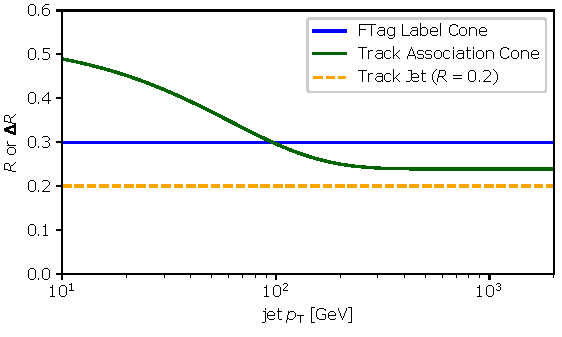
\includegraphics[width=0.5\textwidth]{shrinkCone}
  \caption{The shrinking particle association cone (\hexline{006401}) used to associate muons with a $\DeltaR_\mathrm{\mu, jet}$ smaller than the cone depending on the transverse momentum of the jet. Adopted from \citep{Jacobs:2697316}. }
  \label{fig:shrinkCone}
\end{figure}
Selected muons must be combined muons meaning they are reconstructed using both the inner detector and the muon spectrometer. The closest muon within $\DeltaR_\mathrm{\mu, jet} < 0.4$ to the jet axis is chosen provided it has a minimum \pt of \qty{4}{GeV}. This threshold is set as muon reconstruction below \qty{3}{GeV} is generally unreliable due to minimally ionizing particles losing approximately \qty{3}{GeV} in the ATLAS calorimeters \citep{expectedPerformanceAtlas}.

Truth studies revealed that most muons associated to jets result from secondary (non-prompt) decays of $c$- and $b$-hadrons as as evidenced in figure \ref{fig:muonTruth}(a). However this figure also reveals the introduction of $b$-tagging backgrounds since muons are also associated to light jets. These backgrounds predominantly arise from in flight decays of pions and kaons but also prompt muons from nearby $W$-boson decays and muons from light and strange mesons as shown in figure \ref{fig:muonTruth}(b).
\begin{figure}[htbp]
  \centering
  \subfigure[]{
    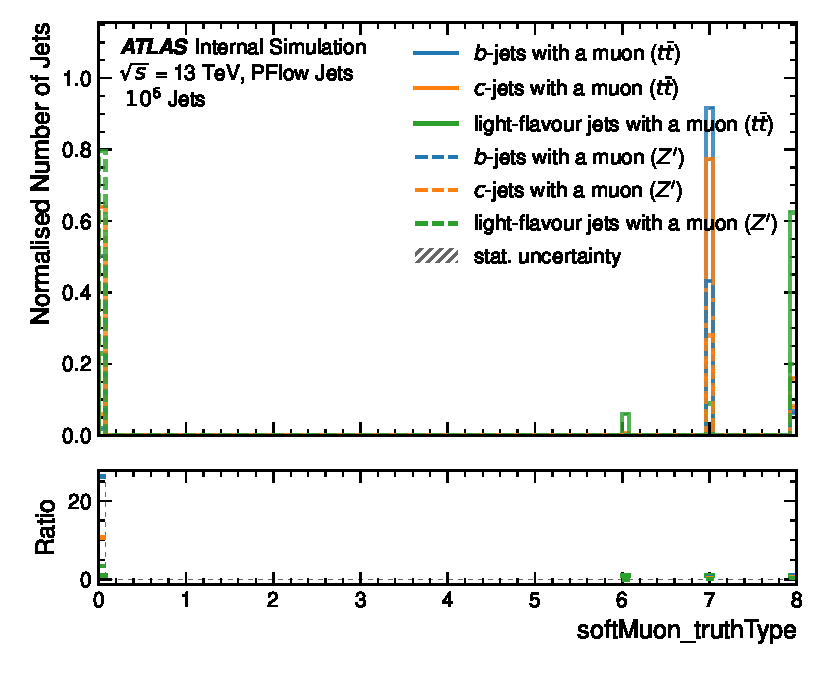
\includegraphics[width=0.47\textwidth]{softMuon_truthType_norm}
  }
  \subfigure[]{
    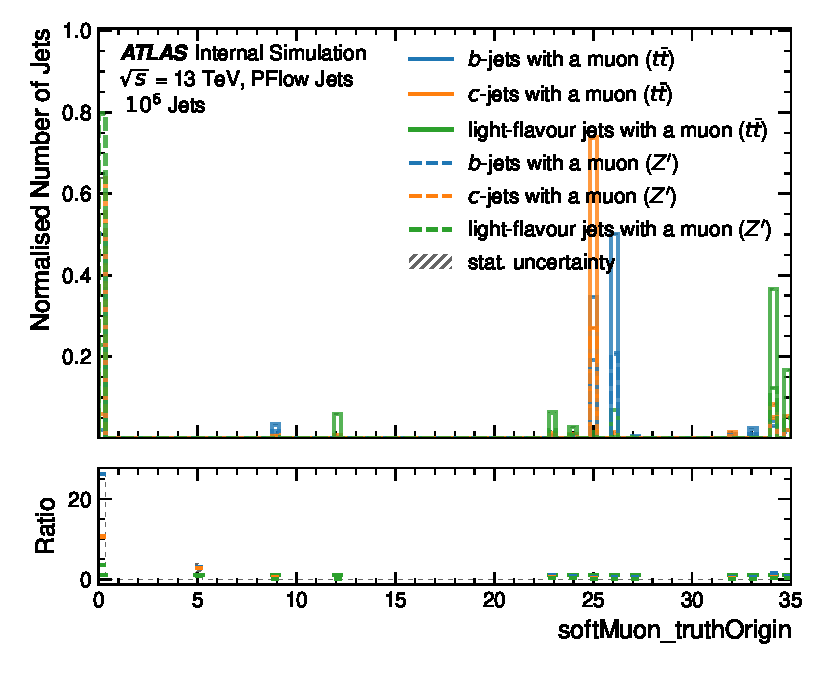
\includegraphics[width=0.47\textwidth]{softMuon_truthOrigin_norm}
  }
  \caption{Jet truth type (a) and truth origin (b) for jets with an associated muon normalized per flavor from $t\overline{t}$ and $Z'$ samples. Truth types: unclassified (0), prompt (6), non-prompt (7) and background muon (8). Truth origins: tau lepton decays (9), prompt muons from nearby W decays (12), light (23), strange (24), charm (25), bottom (26) mesons and in flight decays of pions (34) and kaons (35) according to the Monte Carlo truth classification \citep{mctruthclassification}.}
  \label{fig:muonTruth}
\end{figure}
Table \ref{tab:MuonJetFlavors} shows the proportion of jets with an associated muon for each flavor. Approximately \qty{15}{\percent} of $b$-jets and around \qty{1}{\percent} of both light and tau jets have an associated muon.
\begin{table}[htbp]
  \caption{Fraction of associated muons per flavor. The large fraction for $b$-jets compared to the other flavors is the reason why muons are a useful discriminator for $b$-tagging. }
  \label{tab:MuonJetFlavors}
  \centering
  \begin{tabular}{ l c }
    \hline
    Jet flavor & Fraction of jets with an associated muon \\
    \hline
    light      & 0.0134                                   \\
    c          & 0.0472                                   \\
    b          & 0.1490                                   \\
    tau        & 0.0138                                   \\
    \hline
  \end{tabular}
\end{table}
Figure \ref{fig:muon_2d_truth} visualizes the amount of fake muons in $b$-jets with an associated muons depending on the jet- and muon-\pt. A notable trend is that $b$-jets with low momentum tend to have low momentum muons. Falsely associated muons become more common at high jet momentum and low muon momentum.
\begin{figure}[htbp]
  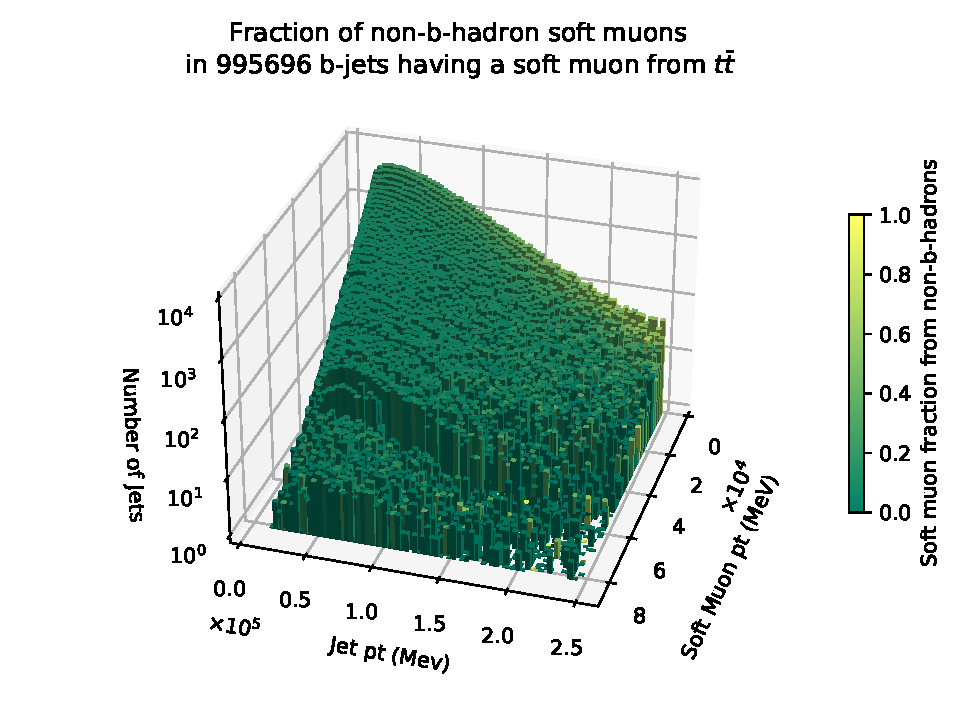
\includegraphics[width=1\textwidth]{muon_2d_truth_ttbar}
  \caption{2D histograms of $p_\mathrm{T}^\mathrm{jet}$ and $p_\mathrm{T}^\mathrm{muon}$ for $t\bar{t}$ selected on $b$-jets only. The colorbar is the fraction of muons that do not originate from b-hadrons. The distributions are actually smooth although some irregularities are visible which is due to a bug in the plotting library.}
  \label{fig:muon_2d_truth}
\end{figure}



\section{Soft Muon Variables}
\label{sec:SoftMuonVariables}
The soft muon variables are selected based on their $b$-tagging discrimination power. The impact parameters of jets as described in section \ref{sec:b_tagging} are determined with the three dimensional impact parameter algorithm (IP3D) detailed in \citep{ATL-PHYS-PUB-2017-013} and are shown in figure \ref{fig:softMuon_ip3dD0}-\ref{fig:softMuon_ip3dZ0Significance}.
\begin{figure}[htbp]
  \centering
    \subfigure[]{
      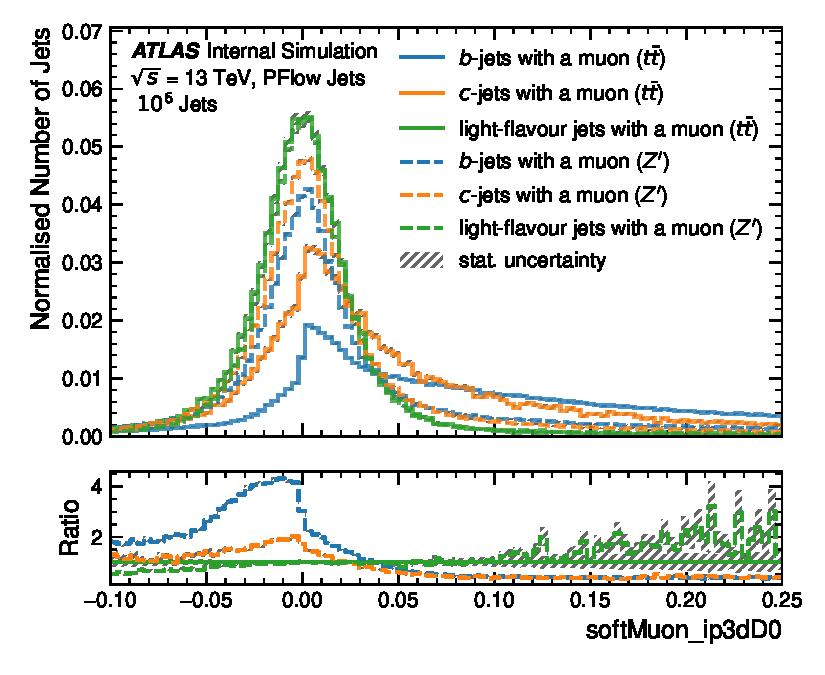
\includegraphics[width=0.47\textwidth]{softMuon_ip3dD0}
      \label{fig:softMuon_ip3dD0}
    }
    \subfigure[]{
      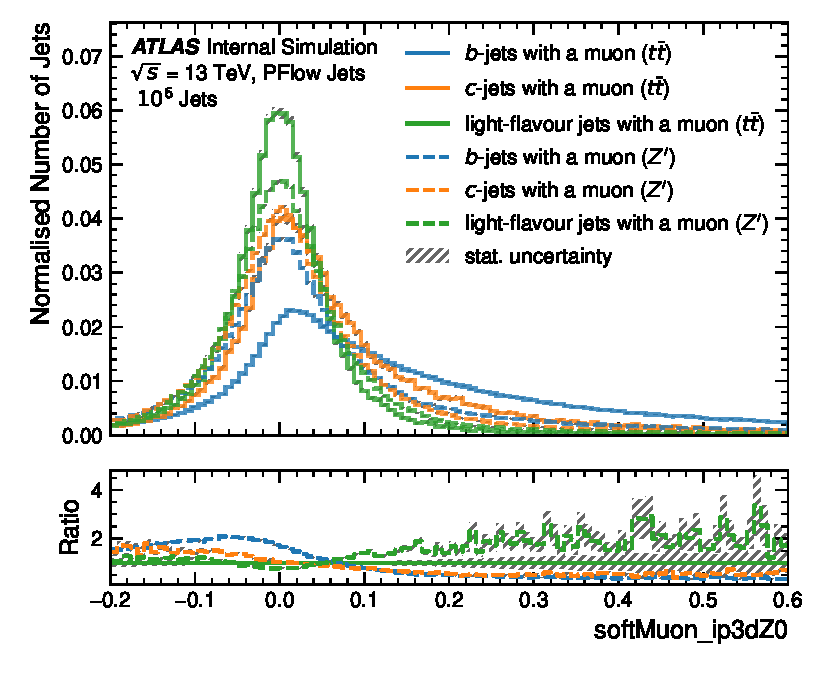
\includegraphics[width=0.47\textwidth]{softMuon_ip3dZ0}
      \label{fig:softMuon_ip3dZ0}
    }
    \\
    \subfigure[]{
      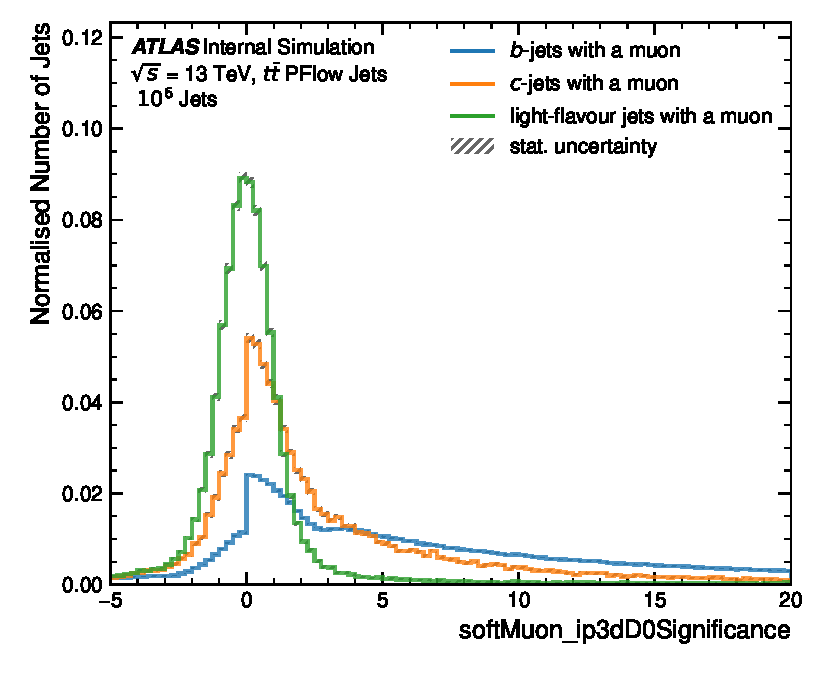
\includegraphics[width=0.47\textwidth]{softMuon_ip3dD0Significance}
      \label{fig:softMuon_ip3dD0Significance}
    }
    \subfigure[]{
      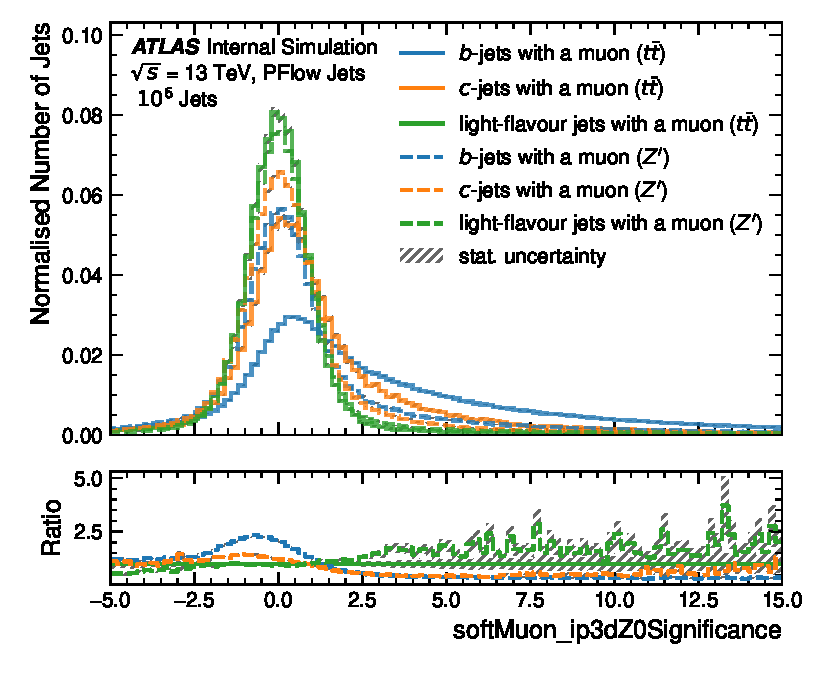
\includegraphics[width=0.47\textwidth]{softMuon_ip3dZ0Significance}
      \label{fig:softMuon_ip3dZ0Significance}
    }
  \caption{Impact parameters of the soft muon retrieved with the IP3D algorithm \citep{ATL-PHYS-PUB-2017-013}, normalized per flavor.}
  \label{fig:softMuonKinematics}
\end{figure}
In addition variables are used to reject muons from in flight decays of Kaons and Pions \citep{ATLAS-CONF-2020-030}. The Scattering Neighbor Significance measures if the track of a particle has kinks that could be a sign of an additional decay. By connecting neighboring detector hits along the track with straight lines and measuring the angles between adjacent lines the Scattering Neighbor Significance is obtained by taking the maximum of the angle divided by its uncertainty. In figure \ref{fig:softMuon_scatteringNeighbourSignificance} light jets therefore tend to have larger values as they have a smaller \pt (cf. figure \ref{fig:softMuon_pt}). Another variable to identify possible background sources is the Momentum Balance Significance. It calculates the difference of the muon-\pt determined with the inner detector with the one from the muon spectrometer and corrects it for energy deposits in the calorimeters. This would be zero in figure \ref{fig:softMuon_momentumBalanceSignificance} for a perfect energy loss correction and if the muon did not arise from an in flight decay. Furthermore there is the curvature comparison between inner detector (ID) and the one from the muon spectrometer (MS) termed q over p ratio: $(q/p)_\mathrm{ID}\, \bm{/}\, (q/p)_\mathrm{MS}$ in figure \ref{fig:softMuon_qOverPratio}. 

\begin{figure}[htbp]
  \centering
    \subfigure[]{
      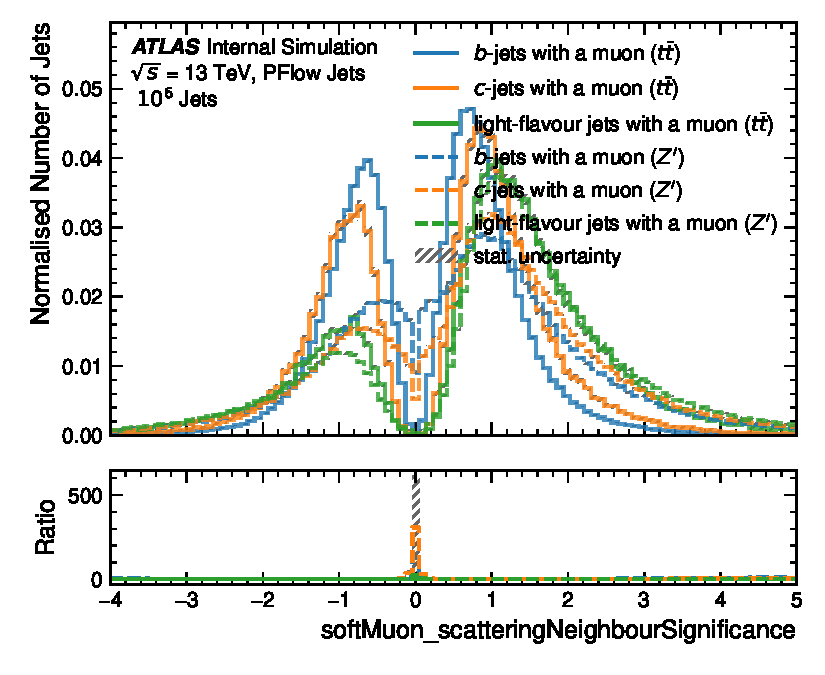
\includegraphics[width=0.47\textwidth]{softMuon_scatteringNeighbourSignificance}
      \label{fig:softMuon_scatteringNeighbourSignificance}
    }
    \subfigure[]{
      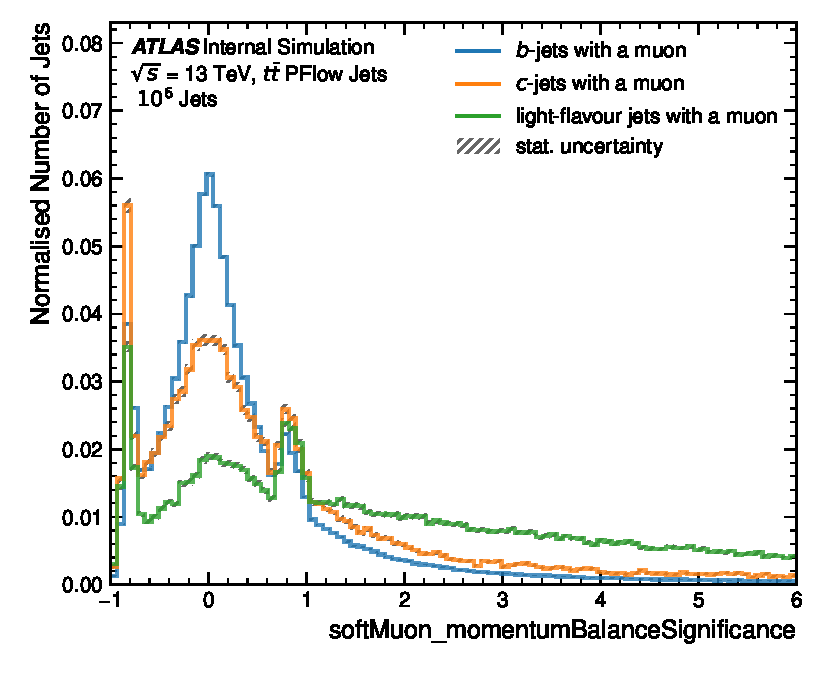
\includegraphics[width=0.47\textwidth]{softMuon_momentumBalanceSignificance}
      \label{fig:softMuon_momentumBalanceSignificance}
    }
    \\
    \subfigure[]{
      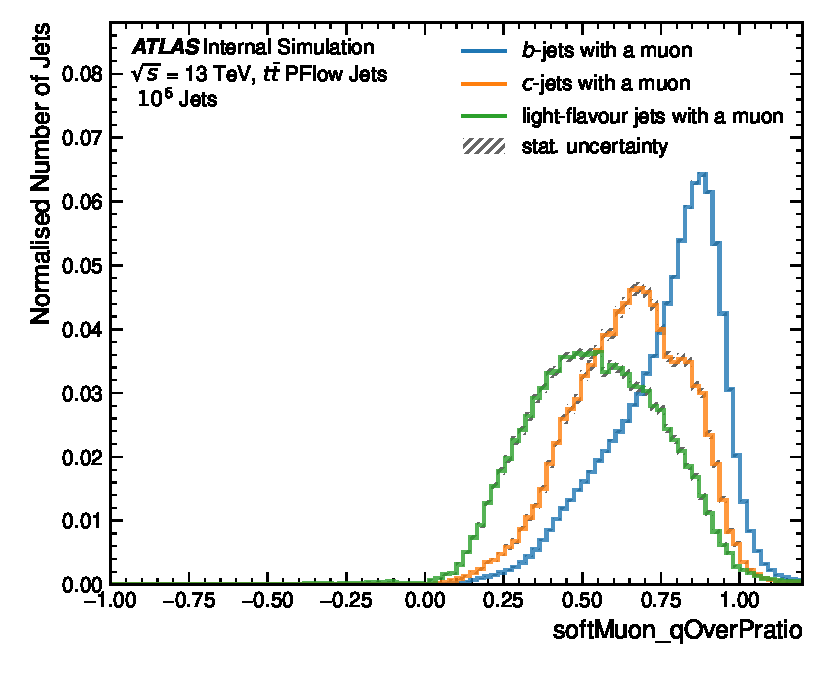
\includegraphics[width=0.47\textwidth]{softMuon_qOverPratio}
      \label{fig:softMuon_qOverPratio}
    }
  \caption{Variables to reject light jet background. Description in section \ref{sec:SoftMuonVariables}.}
  \label{fig:softMuonVariables2}
\end{figure}


\subsection{Adding muons to $b$-tagging algorithms}
Current $b$-tagging algorithms in use are deep feed-forward neural networks with the prefix DL1 that assign a score ($p_\mathrm{b}, p_\mathrm{c}, p_\mathrm{light}$) to a jet depending on its flavor content. Depending on the strategy used to introduce additional tracking information associated with the jet it can become DL1r if the outputs of the RNNIP (Recurrent Neural Network Impact Parameter) \citep{Gilles:2806947} tagger or DL1d if the outputs of the DIPS (Deep Impact Parameter Sets) \citep{ATL-PHYS-PUB-2020-014} tagger are added as inputs to DL1. The ouputs of these taggers are then combined into a signal to background ratio variable, the discriminant
\begin{equation}
  \mathrm{D}=\ln\left(\frac{p_b}{f_c \cdot p_c + (1-f_c)\cdot p_\mathrm{light} }\right).
\end{equation}
$f_c$ is the fraction of charm jets in the background and can be used to tune the importance of the different background classes ($\sum f_\mathrm{bkg} =1$). 

Information of the selected muon variables are added to these tracking information inclusive taggers as additional inputs. Two ways of introducing the muon information were explored. The first refers to an approach where the muon variables itself were used to train an additional neural network called \ac{smt} with architecture: (soft muon input variables) $\rightarrow$ 3 hidden layers (100, 20, 10) $\rightarrow$ 3 outputs nodes for classification of the jet flavor ($p_\mathrm{b}, p_\mathrm{c}, p_\mathrm{light}$). The output scores of the \ac{smt} are then added as inputs to the DL1 training. The tagger resulting from this method is called DL1r\_SMT. In a second approach the muon variables were added directly as inputs to the DL1r training and are referred to here as DL1rmu. The resulting discriminant comparing DL1d and DL1dmu is depicted in Fig. \ref{fig:scores_comparison_DL1d_to_DL1dmu}
\begin{figure}[htbp]
  \centering
  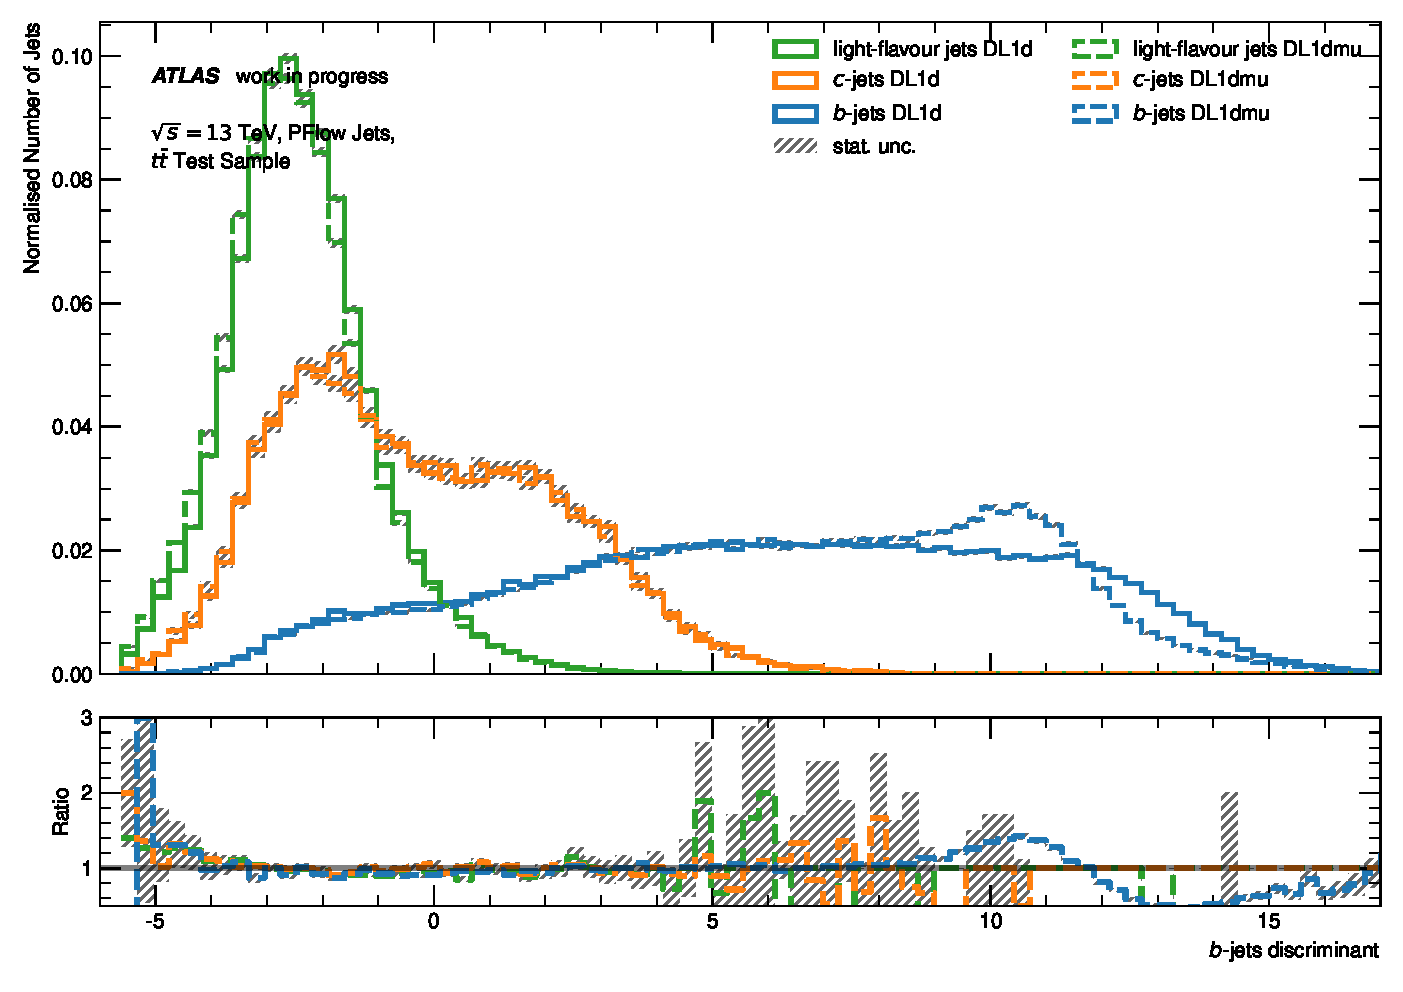
\includegraphics[width=0.6\textwidth]{scores_comparison_DL1d_to_DL1dmu}
  \caption{Discriminant comparison between DL1d ($\bm{\diagup$}) and DL1dmu (\textbf{- -}). The performance of the model increases if the different classes are visually more separated.}
  \label{fig:scores_comparison_DL1d_to_DL1dmu}
\end{figure}


For all trainings the Umami neural network training framework \citep{Froch:2857164} is used with \ttbar and \Zprime Monte Carlo samples described in \citep{ATL-PHYS-PUB-2017-013}. \Zprime is a hypothetical particle used here to enhance the statistics at larger jet-\pt>$\SI{250}{GeV}$. For the training both \ttbar and \Zprime samples are merged and resampled to make the \pt and $\eta$ distributions appear the same for all flavors. This is done to allow for a fair training between flavor categories, as the kinematic regimes are neither over- nor under-represented between flavors when the neural network is trained. The flavor composition of jets can be seen before and after applying the resampling in figure \ref{fig:resampling}.
\begin{figure} 
  \centering
      \subfigure[]{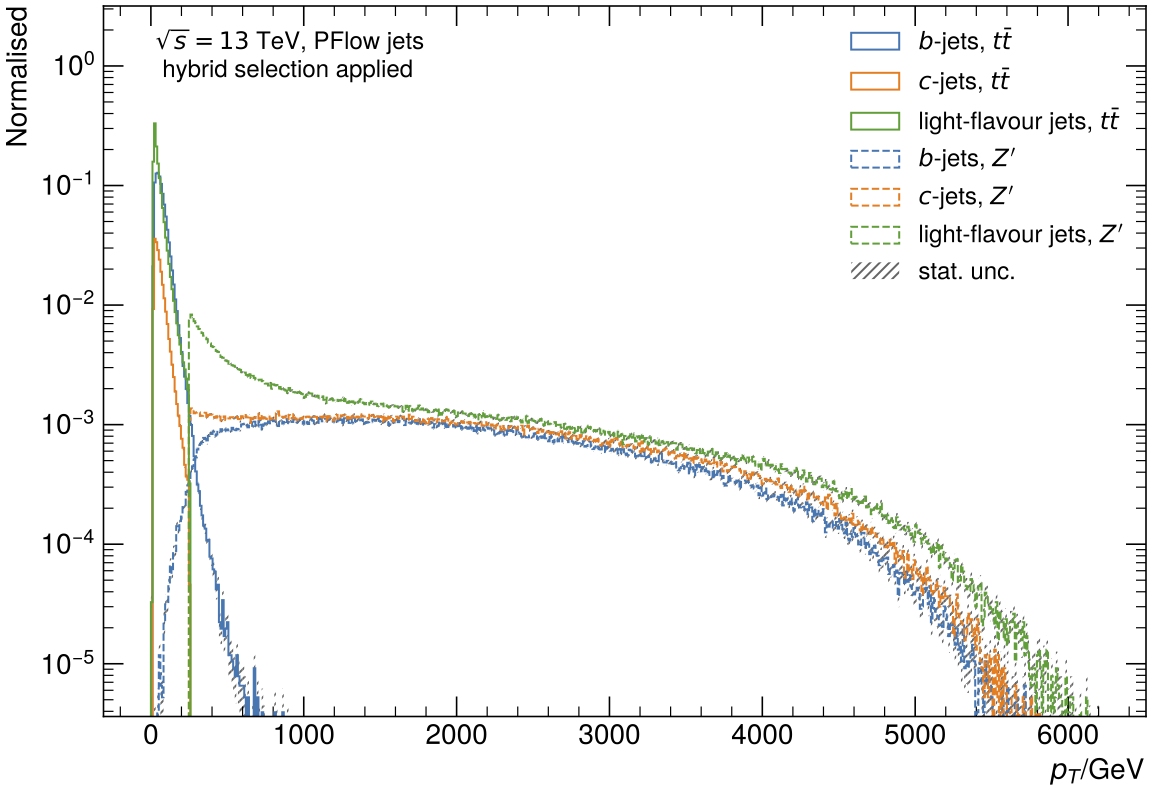
\includegraphics[width=.8\textwidth]{pt_btagJes-cut_spectrum}}\\
      \subfigure[]{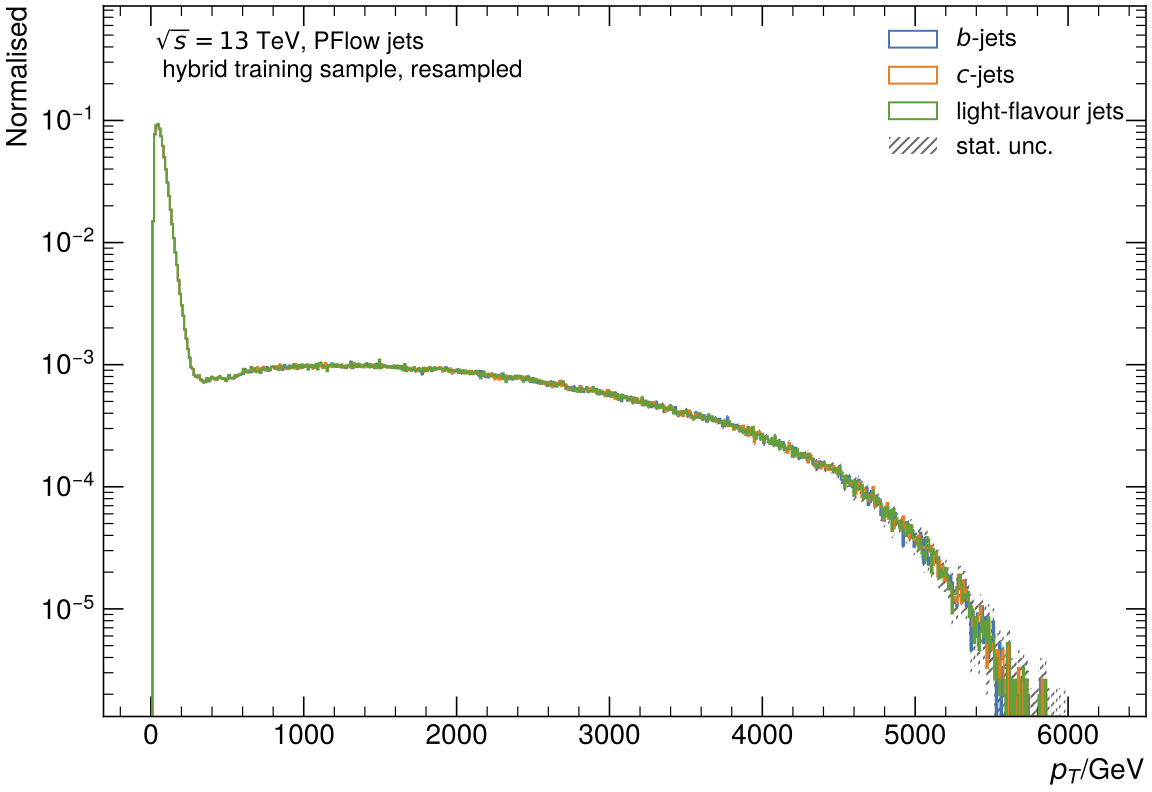
\includegraphics[width=.8\textwidth]{pt_btagJes-downsampled}} 
\caption[]{Jet-\pt per flavor normalized to unity for \ttbar and \Zprime samples \textbf{(a)} before and \textbf{(b)} after resampling. Adopted from \citep{umamiDocs}.}
\label{fig:resampling}    
\end{figure}


% VIVA_13.05.22.pdf ! 


